\documentclass[12pt]{article}

\usepackage[margin=1.5cm]{geometry}        % For setting margins
\usepackage[spanish,es-tabla]{babel}
\selectlanguage{spanish}
\usepackage{amsmath}                % For Math
\usepackage{fancyhdr}                % For fancy header/footer
\usepackage{graphicx}                % For including figure/image
\usepackage{cancel}                    % To use the slash to cancel out stuff in working out equations
\usepackage{amsfonts}
\usepackage{color}
\usepackage{bbm}
\usepackage{float}
\usepackage{subcaption}
\usepackage{lipsum}
\usepackage{listings}
\usepackage{algorithm,algpseudocode}
\usepackage{hyperref}
\usepackage{amssymb}
\usepackage{tikz}
\usepackage{booktabs}
\usetikzlibrary{arrows, positioning}
\captionsetup{compatibility=false}

%%%%%%%%%%%%%%%%%%%%%%
% Set up fancy header/footer
\pagestyle{fancy}
\fancyhead[LO,L]{Alejandro Uribe}
\fancyhead[CO,C]{}
\fancyhead[RO,R]{Aprendizaje Reforzado - Guía 4: Métodos Monte Carlo}
\fancyfoot[LO,L]{}
\fancyfoot[CO,C]{\thepage}
%\fancyfoot[RO,R]{\today}
\renewcommand{\headrulewidth}{0.4pt}
\renewcommand{\footrulewidth}{0.4pt}

\newlength\tindent
\setlength{\tindent}{\parindent}
\setlength{\parindent}{0pt}
\renewcommand{\indent}{\hspace*{\tindent}}
\DeclareMathOperator*{\argmax}{argmax}
\floatname{algorithm}{Algoritmo}

\decimalpoint
\bibliographystyle{ieeetr}
%%%%%%%%%%%%%%%%%%%%%%

\begin{document}
    \indent\underline{\textbf{Ejercicio 1}}\\
\textcolor{green}{[Programación]} Para el proceso de Markov de recompensas (MRP) de la figura~\ref{fig:grafo_ej_1}, calcular los valores de los estados de forma iterativa con los siguientes algoritmos y compare sus convergencias.
Considere factor de descuento $\gamma < 0.9$.\\

\begin{figure}[H]
    \centering
    \begin{tikzpicture}[->, >=stealth', auto, semithick, node distance=2cm]
        % Nodes
        \node[circle, draw] (s1) {$s_1$};
        \node[circle, draw, right=of s1] (s2) {$s_2$};
        % Arrows
        \path (s1) edge[bend left=60] node {R=1} (s2)
              (s2) edge[bend left=60] node[align=center] {R=2 \\ $p(s_2 \mid s_1) = 1$ \\ $p(s_1 \mid s_2) = 1$} (s1);
    \end{tikzpicture}
    \caption{Grafo de transición de estados}\label{fig:grafo_ej_1}
\end{figure}


\begin{itemize}
    \item Actualizar todos los valores a la vez por iteración: $v_{k+1} = r + \gamma P v_k$, con $v_k\, r$ siendo los vectores de valores y recompensas, respectivamente; y $P$ la matriz de probabilidades de transición.
    \item Actualizar los valores de un estado por vez \textit{(in place)}: $v_{k+1}(s') = r(s') + \gamma v_k(s)$, con $v_k(s)$ y $r(s')$ siendo los valores y recompensas correspondientes a los estados $s$ y $s'$, respectivamente.
\end{itemize}

\indent\underline{\textbf{Solución}}\\
La implementación de los algoritmos se realizó en Python, que se puede encontrar en el repositorio de \href{https://github.com/MasterUBA-DM-KD/Aprendizaje_Reforzado/blob/5ae50da937b14f0a11c416e40019a4b5661dd51b/docs/guia/3/notebooks/utils.py}{GitHub}.

Sea, $P$ la matriz de probabilidades de transición:

\[
  P = \begin{bmatrix} 0 & 1 \\ 1 & 0 \end{bmatrix}
\]

Sea $r$ el vector de recompensas:

\[
  r = \begin{bmatrix} 1 \\ 2 \end{bmatrix}
\]

A continuación los resultados de los valores de los estados para $\gamma \in [0, 0.9)$ usando los métodos \textit{iterativo} e \textit{in place}.

\paragraph{Método \textit{iterativo}} Se calculó el vector de valor $v_{k+1}$ usando el cálculo iterativo con la librería \texttt{numpy} de Python\footnotemark.
La figura~\ref{fig:iter_gamma_vk} muestra los valores de $v_{k+1}$ y la figura~\ref{fig:iter_gamma_iter} muestra el número de iteraciones necesarias para converger, ambas para $\gamma \in [0, 0.9)$.

\footnotetext{Se una tolerancia de $10^{-6}$ y un máximo de $1000$ iteraciones.}

La figura~\ref{fig:iter_gamma} muestra los resultados para el método \textit{iterativo}.

\begin{figure}[H]
    \centering
    \begin{subfigure}[H]{0.45\textwidth}
        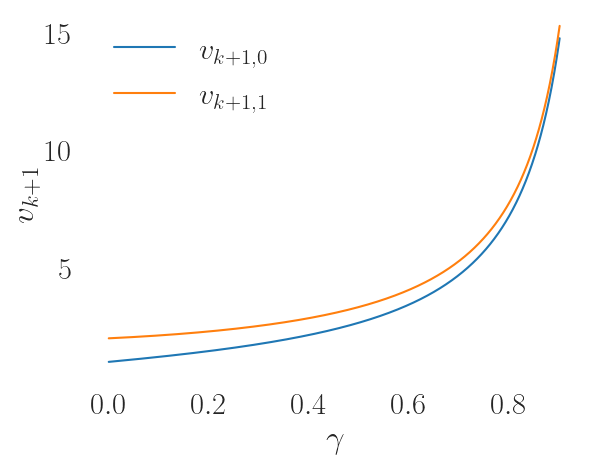
\includegraphics[width=\textwidth]{../img/gamma_v_k}
        \caption{Vector de valores}
        \label{fig:iter_gamma_vk}
    \end{subfigure}
    \begin{subfigure}[H]{0.45\textwidth}
        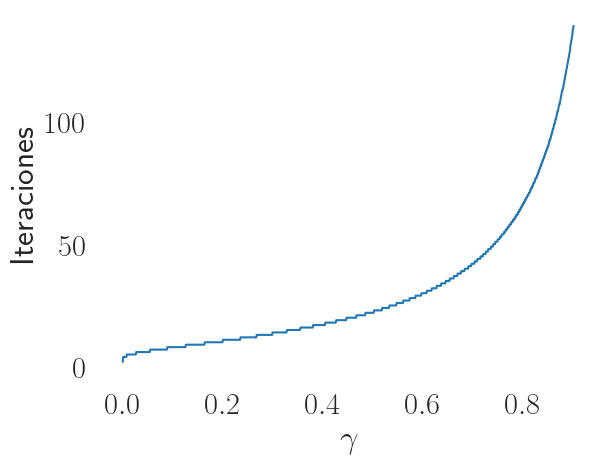
\includegraphics[width=\textwidth]{../img/gamma_iters}
        \caption{Número de iteraciones para converger}
        \label{fig:iter_gamma_iter}
    \end{subfigure}
    \caption{Resultados del método \textit{iterativo}}\label{fig:iter_gamma}
\end{figure}

\paragraph{Método \textit{in place}} Se calculó el vector de valor $v_{k+1}$ usando el cálculo iterativo con la librería \texttt{numpy} de Python\footnotemark.
La figura~\ref{fig:inplace_gamma_vk} muestra los valores de $v_{k+1}$ y la figura~\ref{fig:inplace_gamma_iter} muestra el número de iteraciones necesarias para converger, ambas para $\gamma \in [0, 0.9)$.

\footnotetext{Se fijó una tolerancia de $10^{-6}$ y un máximo de $1000$ iteraciones.}

La figura~\ref{fig:inplace_gamma} muestra los resultados para el método \textit{in place}.

\begin{figure}[H]
    \centering
    \begin{subfigure}[H]{0.45\textwidth}
        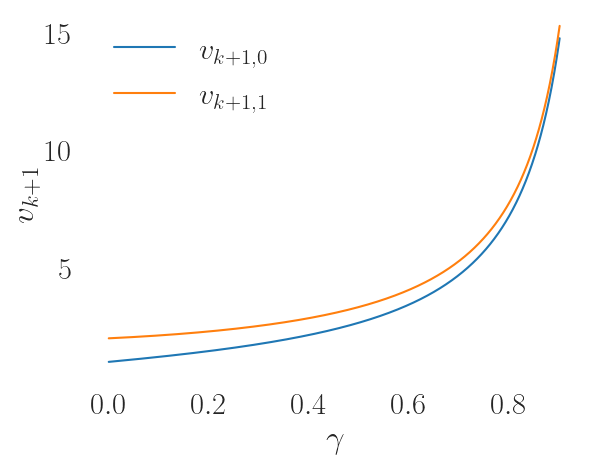
\includegraphics[width=\textwidth]{../img/gamma_v_k}
        \caption{Vector de valores}
        \label{fig:inplace_gamma_vk}
    \end{subfigure}
    \begin{subfigure}[H]{0.45\textwidth}
        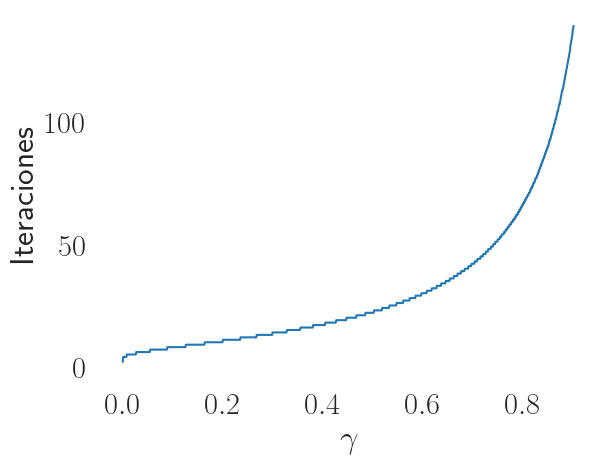
\includegraphics[width=\textwidth]{../img/gamma_iters}
        \caption{Número de iteraciones para converger}
        \label{fig:inplace_gamma_iter}
    \end{subfigure}
    \caption{Resultados del método \textit{inplace}}\label{fig:inplace_gamma}
\end{figure}

\indent\underline{\textbf{Conclusiones}}\\
No existe una diferencia significativa entre los métodos \textit{iterativo} e \textit{in place} para valores de $\gamma \in [0, 0.9)$.
A continuación se presentan las conclusiones de los resultados obtenidos.

\paragraph{Vector de valores $v_{k+1}$}
Las figuras~\ref{fig:iter_gamma_vk} y~\ref{fig:inplace_gamma_vk} muestran los valores de $v_{k+1}$ para $\gamma \in [0, 0.9)$ para los métodos \textit{iterativo} e \textit{in place}, respectivamente.
De las figuras se concluye,

\begin{itemize}
    \item Ambos métodos mostraron una rápida convergencia cuando $\gamma \approx 0$, dando como resultado $v_{k+1} = r = \begin{bmatrix} 1 \\ 2 \end{bmatrix}$.
    \item Los valores de $v_{k+1}$ aumentan de forma exponencial a medida que $\gamma$ aumenta.
    \item Conforme $\gamma \rightarrow 0.9$, los métodos convergen a los valores teóricos $v = \begin{bmatrix} 14.74 \\ 15.26 \end{bmatrix}$.
\end{itemize}

\paragraph{Iteraciones}
Las figuras~\ref{fig:iter_gamma_iter} y~\ref{fig:inplace_gamma_iter} muestran el número de iteraciones necesarias para converger para $\gamma \in [0, 0.9)$ para los métodos \textit{iterativo} e \textit{in place}, respectivamente.
De las figuras se concluye,

\begin{itemize}
    \item Las iteraciones necesarias para converger aumentan de forma exponencial a medida que $\gamma$ aumenta.
    \item Conforme $\gamma \rightarrow 0.9$, se requieren más iteraciones para converger, lo que se traduce en un mayor tiempo de cómputo.
\end{itemize}

\paragraph{Implementación}En cuanto a la implementación de ambos métodos, la diferencia entre el método \textit{iterativo} e \textit{in place} radica en que el segundo no requiere de una matriz de transición $P$.
Desde una perspectiva computacional el método \textit{in place} es más eficiente, ya que no requiere de una matriz de transición.
También es útil en escenarios en los que la matriz de transición no es conocida, como en el caso de un agente que interactúa con un entorno desconocido.

\line(1,0){\textwidth}

    \indent\underline{\textbf{Ejercicio 2}}\\
Demostrar que la política $\varepsilon \text{ - \textit{Greedy}}$, definida de la siguiente manera

\begin{equation}
\pi(a|s) = \left\{
\begin{array}{lcc}
    1 - \varepsilon + \frac{\varepsilon}{|A(s)|} & si  & a = a^{\ast} \\ \\
     \frac{\varepsilon}{|A(s)|} &  si & a \neq a^{\ast}
\end{array}
   \right.\label{eq:equation}
\end{equation}

es una distribución de probabilidad válida, donde $|A(s)|$ es el número de acciones para el estado $s, \ \varepsilon < 1$ es un número positivo pequeño, y $a^{\ast}$ es la acción óptima (decisión greedy) para el estado $s$.
¿Hay que pedir alguna condición sobre $\varepsilon$?

\indent\underline{\textbf{Solución}}\\

\line(1,0){\textwidth}

    \indent\underline{\textbf{Ejercicio 3}}\\
En el Ejemplo 4.1 (\textit{GridWorld}, Sutton\&Barto, 2018)~\cite{Sutton2018}, suponga que se agrega un nuevo estado $15$ debajo del estado $13$ y sus acciones: \textit{left, up, right} y \textit{down}, lleva al agente a los estados $12$, $13$, $14$ y $15$, respectivamente.

\begin{itemize}
    \item Considere que las transiciones desde los estados originales no se cambian.
    ¿Cuánto vale $v_{\pi}(15)$ para la política $\pi$ aleatoria y equiprobable?
    Utilice $v(12) = -22$, $v(13) = -20$, $v(14) = -14$ (figura~\ref{fig:gridworld}).
\end{itemize}

Justifique su respuesta.

\indent\underline{\textbf{Solución}}\\
Sea,\\
$p(s',r|s,a) = 0.25, \ \forall s \in S, \forall a \in A$\\

La función de valor de estado $v_{\pi}(s)$ para la política $\pi$ es:

\[
    v_{pi} = \sum_{a} \pi(a|s) \sum_{s',r} p(s',r|s,a) \left[ r + \gamma v_{\pi}(s') \right]
\]

Para calcular $v_{\pi}(15)$,

\begin{align*}
    v_{\pi}(15) &= \sum_{a} \pi(a|15) \sum_{s',r} p(s',r|15,a) \left[ r + \gamma v_{\pi}(s') \right] \\
    &= 0.25 \left[ r + \gamma v_{\pi}(s') \right] \\
    &= 0.25 \left[\left(-1 -20 \right) + \left(-1 -22 \right) + \left(-1 -14 \right) + \left(-1 + v_{\pi}(15) \right) \right] \\
    &= 0.25 \left[ -21 -23 -15 -1 + v_{\pi}(15) \right] \\
    &= 0.25 \left[ -60 + v_{\pi}(15) \right] \\
    &= -15 + 0.25 \cdot v_{\pi}(15)
\end{align*}

Al considerar que las transiciones desde los estados originales no se cambian, es posible la transición del estado $13$ al $15$.
Pasar al estado $15$ tiene un valor igual al del estado $13$.
Por lo tanto,

\begin{align*}
    v_{\pi}(15) &= v_{\pi}(13) \\
    &= -20
\end{align*}

Al reemplazar $v_{\pi}(15)$ en la ecuación anterior, se obtiene:

\begin{align*}
    v_{\pi}(15) &= -15 + 0.25 \cdot v_{\pi}(15) \\
    &= -15 + 0.25 \cdot (-20) \\
    &= -15 - 5 \\
    &= -20
\end{align*}

\line(1,0){\textwidth}

    \indent\underline{\textbf{Ejercicio 4}}\\
En el Ejemplo 4.3 (\textit{Gambler’s problem, Sutton\&Barto, 2018})~\cite{Sutton2018}, la política óptima tiene una forma particular (ver figura~\ref{fig:gamblers_problem}) con máximo en $50$.
Es decir, cuando el jugador tiene $\$50$, le conviene apostarlo todo; sin embargo, cuando tiene $\$51$, le conviene apostar $\$1$.
¿Por qué sucede esto?

\begin{figure}[H]
    \centering
    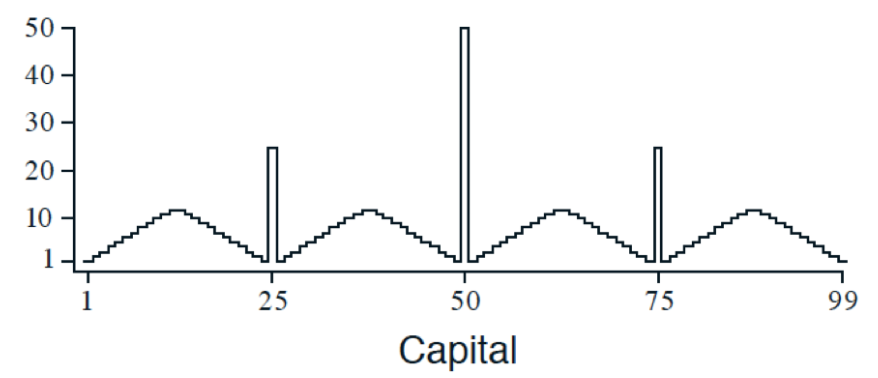
\includegraphics[width=0.5\textwidth]{../img/gamblers_problem}
    \caption{Ejemplo 4.3~\cite{Sutton2018}}
    \label{fig:gamblers_problem}
\end{figure}

\indent\underline{\textbf{Solución}}\\
El ejemplo 4.3 (\textit{Gambler’s problem, Sutton\&Barto, 2018})~\cite{Sutton2018} se plantea como un MDP finito, sin descuento, episódico y con un conjunto de estados $s \in \left\{0, 1, \ldots, 99\right\}$ y un conjunto de acciones $a \in \left\{0, 1, \ldots, \min(s, 100-s)\right\}$.

Por otro lado, la política final encontrada es tal que $p_h=0.4$, es decir, la probabilidad de que la moneda salga cara es $0.4$.

Por lo tanto, cuando la moneda está cargada y al jugador le conviene minimizar el número de apuestas realizadas porque en el largo plazo, el jugador perderá dinero.
Por lo tanto, el jugador tiene una \textit{ventaja}\footnotemark y le conviene apostar todo cuando tiene $\$50$, ya que a la izquierda y derecha de este valor las apuestas llevarán al jugador de vuelta a $\$50$.
Por lo que si tiene $\$51$ le conviene apostar $\$1$ sabiendo que si pierde, volverá a $\$50$.
\footnotetext{La ventaja se refiere a que si el jugador apuesta los $\$50$ tendrá el $40\%$ de probabilidad de ganar.}

\line(1,0){\textwidth}

    \indent\underline{\textbf{Ejercicio 5}}\\
\textcolor{green}{[Programación]} Implemente el Algoritmo de Iteración de Valores para el el Ejemplo 4.3 (\textit{Gambler’s problem, Sutton\&Barto, 2018})~\cite{Sutton2018} para los siguientes casos:

\begin{itemize}
    \item $p_h = 0.25$.
    \item $p_h = 0.55$.
\end{itemize}

Compare los resultados y saque conclusiones.

\indent\underline{\textbf{Solución}}\\
La implementación de los algoritmos se realizó en Python, que se puede encontrar en el repositorio de \href{https://github.com/MasterUBA-DM-KD/Aprendizaje_Reforzado/blob/5ae50da937b14f0a11c416e40019a4b5661dd51b/docs/guia/3/notebooks/utils.py}{GitHub}.

Sea,\\
$N=100$: capital máximo\\
$S=\left\{0, 1, \ldots, 100\right\}$: conjunto de estados\\
$A=\left\{0, 1, \ldots, \min(s, 100-s)\right\}$: conjunto de acciones\\

El Algoritmo de Iteración de Valores para el Ejemplo 4.3 (\textit{Gambler’s problem, Sutton\&Barto, 2018})~\cite{Sutton2018} se implementó en Python\footnotemark.
A continuación, los resultados de la implementación, $p_h = 0.25$, se muestran en las figuras~\ref{fig:ph_025_sweeps} y~\ref{fig:ph_025_policy}.

\footnotetext{Se fijó una tolerancia de $10^{-3}$ para la convergencia.}

\begin{figure}[H]
    \centering
    \begin{subfigure}[H]{0.45\textwidth}
        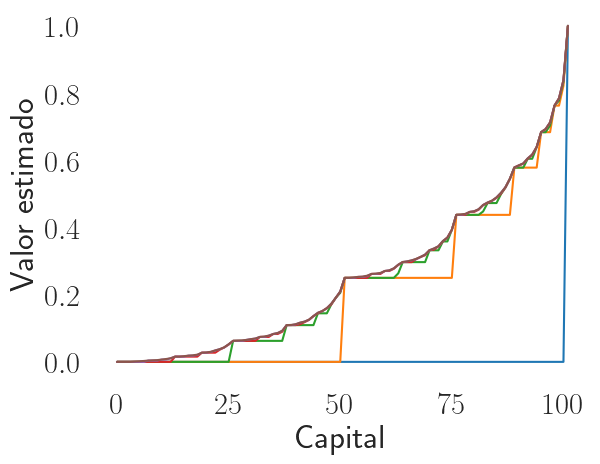
\includegraphics[width=\textwidth]{../img/sweeps_0.25}
        \caption{$sweeps \in [0, N]$}
        \label{fig:ph_025_sweeps}
    \end{subfigure}
    \begin{subfigure}[H]{0.45\textwidth}
        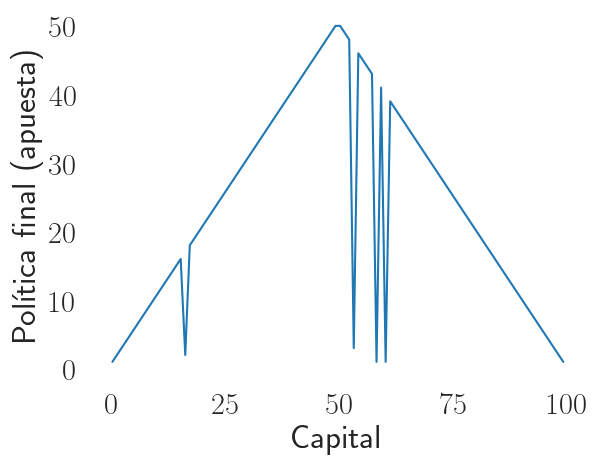
\includegraphics[width=\textwidth]{../img/policy_0.25}
        \caption{Política final}
        \label{fig:ph_025_policy}
    \end{subfigure}
    \caption{$ph=0.25$}
    \label{fig:ph_025_gamblers_problem}
\end{figure}

A continuación, los resultados de la implementación, $p_h = 0.55$, se muestran en las figuras~\ref{fig:ph_055_sweeps} y~\ref{fig:ph_055_policy}.

\begin{figure}[H]
    \centering
    \begin{subfigure}[H]{0.45\textwidth}
        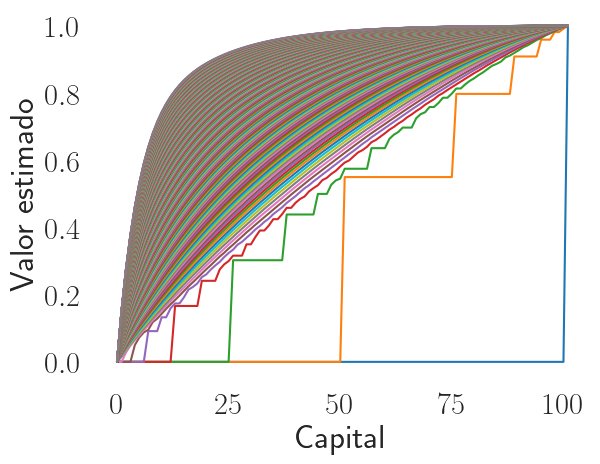
\includegraphics[width=\textwidth]{../img/sweeps_0.55}
        \caption{$sweeps \in [0, N]$}
        \label{fig:ph_055_sweeps}
    \end{subfigure}
    \begin{subfigure}[H]{0.45\textwidth}
        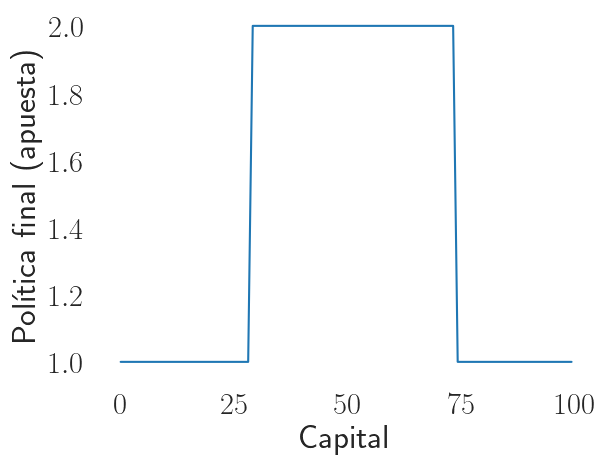
\includegraphics[width=\textwidth]{../img/policy_0.55}
        \caption{Política final}
        \label{fig:ph_055_policy}
    \end{subfigure}
    \caption{$ph=0.55$}
    \label{fig:ph_055_gamblers_problem}
\end{figure}

\indent\underline{\textbf{Conclusiones}}
\paragraph{Convergencia} En las figuras~\ref{fig:ph_025_sweeps} y~\ref{fig:ph_055_sweeps} se muestra que a medida que se aumentan las iteraciones (sweeps), los valores de vada estado convergen a un valor estable.

\paragraph{Política final} Se encuentra influenciada por el valor de $p_h$.
Cuando la probabilidad de ganar es baja la política óptima es apostar poco, especialmente cuando el capital es bajo, hecho que se deba al alto riesgo de perder el capital.
Además, para este caso la política final tiene forma de \textit{V} invertida como se muestra en la figura~\ref{fig:ph_025_policy}.

Por otro lado, cuando la probabilidad de ganar es alta, la política óptima es apostar más, especialmente cuando el capital es intermedio, hecho que se debe a la alta probabilidad de ganar y la posibilidad de maximizar la ganancia.
Además, para este caso la política final tiene forma de \textit{V} achatada, como se muestra en la figura~\ref{fig:ph_055_policy}.

En ambos casos:
\begin{itemize}
    \item Se apuesta poco si se tiene poco capital para evitar perderlo.
    \item Se apuesta más si se tiene un capital intermedio, aprovechando la oportunidad de ganar.
    \item Se apuesta poco si se tiene mucho capital para asegurar ganancia.
\end{itemize}

Se hace la salvedad que en el caso de $p_h = 0.25$ la política final tiene un máximo en el que se encuentra poca estabilidad.

\line(1,0){\textwidth}

    \indent\underline{\textbf{Ejercicio 6}}\\
Demostrar la ecuación de \textit{Bellman} para MRPs con $N$ estados

\[
    v = r + \gamma Pv,
\]

donde $v \in \mathbb{R}^N$ es el vector de valores de estados, $r \in \mathbb{R}^N$ es el vector de recompensas medias partiendo de cada estado, $P \in \mathbb{R}^{N \times N} $ es la matriz de transiciones y $\gamma$ es el factor de descuento.

\indent\underline{\textbf{Solución}}\\
Sea,\\
$v \in \mathbb{R}^N$: Vector de valores de estados.\\
$r \in \mathbb{R}^N$: Vector de recompensas medias partiendo de cada estado.\\
$P \in \mathbb{R}^{N \times N}$: Matriz de transiciones.\\
$\gamma \in \left[0,1\right)$: Factor de descuento. \\
$i$: Índice del estado.

Partiendo de la ecuación de \textit{Bellman} para un estado $i$,

\[
    v_i = r_i + \gamma \sum_{j=1}^{N} P_{ij} v_j
\]

Es decir, el valor de un estado $i$ es la recompensa inmediata $r_i$ más el valor esperado de los estados siguientes ponderados por la probabilidad de transición desde $i$ a $j$, $P_{ij}$, siendo la matriz de transiciones, y descontados por el factor $\gamma$.
El primer término se puede expresar en forma matricial como,

\[
    r
\]

El segundo término es la suma ponderada de los valores de los estados siguientes.

\[
    \gamma \sum_{j=1}^{N} P_{ij} v_j
\]

Es decir, el factor de descuento $\gamma$ resta valor a los estados futuros~\cite{Sutton2018}.
Este término se puede expresar en forma matricial como,

\[
    \gamma Pv
\]

Al sumar ambos términos se obtiene la ecuación de \textit{Bellman} para MRPs con $N$ estados,

\[
    v = r + \gamma Pv
\]

\line(1,0){\textwidth}

    \bibliography{references}

\end{document}
